\section{Chest Disease Detection Model}
Chest diseases remain among the leading causes of morbidity and mortality worldwide, placing a significant burden on healthcare systems and emphasizing the need for accurate and timely diagnosis. Medical imaging, particularly chest X-ray imaging, plays a vital role in the detection and assessment of respiratory diseases such as COVID-19, Tuberculosis, and Pneumonia. However, manual interpretation of chest radiographs can be time-consuming and may be subject to variability among radiologists, especially in high-demand clinical environments.

Recent advances in Artificial Intelligence (AI) and Deep Learning have demonstrated remarkable potential in assisting medical professionals by automatically analyzing medical images and identifying disease-related patterns. In this context, this project presents a Chest Disease Detection Model designed to classify chest X-ray images and detect the presence of three major respiratory diseases: COVID-19, Tuberculosis, and Pneumonia.

Unlike traditional multi-class classification approaches, these diseases are not mutually exclusive and may coexist within the same patient. Therefore, the proposed system is formulated as a multi-label classification problem, allowing the model to predict one or more diseases simultaneously from a single chest X-ray image. This approach better reflects real-world clinical scenarios and enhances the model's applicability in practical healthcare settings.

The primary objective of this model is to provide an intelligent and reliable diagnostic support tool that can assist healthcare professionals in the early detection and screening of chest diseases. By leveraging deep learning techniques and medical imaging data, the system aims to improve diagnostic efficiency, support clinical decision-making, and contribute to better patient outcomes.

\subsection{Motivation}
Respiratory diseases represent one of the most formidable challenges confronting modern healthcare systems worldwide. Conditions such as COVID-19, Pneumonia, and Tuberculosis (TB) collectively account for millions of deaths and hospitalizations annually, placing enormous strain on healthcare infrastructure, particularly in low- and middle-income countries where access to experienced radiologists and advanced diagnostic facilities remains severely limited. The timely and accurate diagnosis of these conditions is critical, since delayed or erroneous diagnoses can result in inappropriate treatment, accelerated disease progression, and preventable mortality.

Chest X-ray (CXR) imaging remains the cornerstone of respiratory disease diagnosis owing to its widespread availability, low cost, and rapid turnaround time. However, the visual interpretation of chest radiographs is a highly complex, skill-intensive task that demands years of specialized training. Even seasoned radiologists can face considerable difficulty when attempting to differentiate between visually similar pathologies, such as COVID-19 pneumonitis and bacterial pneumonia, or when interpreting images of suboptimal quality obtained in resource-constrained settings. Furthermore, the global shortage of trained radiologists, particularly during large-scale health crises such as the COVID-19 pandemic, has created an unprecedented demand for automated, reliable, and scalable diagnostic support tools.

Recent advances in deep learning, and in particular convolutional neural networks (CNNs), have demonstrated transformative potential in the field of medical image analysis. Architectures such as DenseNet, ResNet, and EfficientNet have achieved or surpassed radiologist-level performance on several benchmark medical imaging tasks. These developments motivate a comprehensive investigation into the deployment of deep learning frameworks for the simultaneous, multi-class differentiation of the most clinically prevalent chest diseases.

Beyond the challenge of multi-class classification itself, a further compelling motivation exists for the application of \textbf{Federated Learning (FL)} within this domain. Medical data is inherently sensitive and subject to stringent privacy regulations, including HIPAA and GDPR, which impose significant restrictions on the centralized aggregation of patient-level imaging data across different hospitals or jurisdictions. Federated Learning offers an elegant solution to this dilemma by enabling collaborative model training across multiple distributed nodes — each representing a hospital or imaging center — without ever requiring raw patient data to leave its local environment.

Finally, the integration of \textbf{Explainable Artificial Intelligence (XAI)} techniques, specifically Gradient-weighted Class Activation Mapping (Grad-CAM), addresses the critical concern of model interpretability in clinical settings. A "black-box" deep learning model, regardless of its accuracy, is unlikely to gain the trust of clinical practitioners unless its decision-making process can be visualized and verified. By producing saliency maps that highlight the anatomical regions most influential to the model's predictions, Grad-CAM bridges the gap between algorithmic performance and clinical trustworthiness.

Taking together, these motivations drive the design of a comprehensive, privacy-preserving, and interpretable deep learning pipeline for the automated classification of chest diseases, which constitutes the core contribution of this project.

\subsection{Problem Statement}
\label{sec:chest_challenges}
The central challenge addressed in this work is the development of a robust, generalizable, and clinically trustworthy deep learning system capable of accurately distinguishing between four clinically significant chest conditions from standard posterior-anterior (PA) or AP chest radiographs. The four target classes are:

\begin{itemize}
	\item \textbf{COVID-19:} A viral pneumonia caused by SARS-CoV-2, characterized on CXR by bilateral, peripheral ground-glass opacities and consolidations, predominantly in the lower lobes.
	\item \textbf{Pneumonia: }: Bacterial or viral pneumonia presenting as airspace consolidation, often lobar or segmental, with air bronchograms and pleural effusion in more severe cases.
	\item \textbf{Tuberculosis (TB): }A chronic bacterial infection by Mycobacterium tuberculosis, displaying a wide spectrum of CXR patterns including upper-lobe infiltrates, cavities, fibrosis, hilar lymphadenopathy, and miliary nodules.
	\item \textbf{Normal: }Healthy subjects with no discernible pulmonary pathology on the radiograph.
\end{itemize}

The specific problems this project aims to solve are enumerated below:

\begin{enumerate}
	\item \textbf{Multi-class classification under class imbalance:} The dataset exhibits natural imbalances between classes, which must be addressed through appropriate class-weighting and augmentation strategies to prevent model bias toward over-represented classes.
	\item \textbf{Differentiation of visually similar pathologies:} COVID-19 and Pneumonia share substantial radiological overlap, making their discrimination a particularly challenging sub-problem. The system must learn discriminative, class-specific features rather than coarse, general patterns.
	\item \textbf{Lung region isolation: }The presence of non-pulmonary structures (ribs, heart shadow, diaphragm, spine, clavicles) in raw CXR images can mislead the classifier toward irrelevant features. A dedicated lung segmentation stage using U-Net is therefore proposed to restrict the model's attention to pulmonary anatomy.
	\item \textbf{Privacy-preserving distributed training: } In a realistic multi-hospital deployment scenario, patient data cannot be pooled centrally. The system must achieve competitive performance under a federated training paradigm with 2, 3, or 4 participating clients, each holding only a partition of the global dataset.
	\item \textbf{Model interpretability:} The system must be able to generate visual explanations for each prediction, enabling clinicians to verify that the model is attending to diagnostically meaningful regions of the radiograph.
\end{enumerate}
Formally, the classification task can be stated as follows: given an input chest radiograph 
$x \in \mathbb{R}^{H \times W \times C}$ and a label space 
$\mathcal{Y} = \{\text{COVID-19}, \text{Normal}, \text{Pneumonia}, \text{Tuberculosis}\}$, 
the objective is to learn a mapping

\[
f : x \mapsto \hat{y}
\]

that minimizes the expected classification error

\[
\mathbb{E}\left[\mathcal{L}(f(x), y)\right]
\]

over the joint distribution of images and labels, whilst satisfying the constraints of data privacy and clinical interpretability.

\subsection{Model Architecture Overview}
The proposed system is a multi-stage deep learning pipeline designed to address each of the challenges outlined in Section~\ref{sec:chest_challenges}. The pipeline is structured into four principal stages, each of which transforms the input data progressively toward the final classification decision. Figure~\ref{fig:chest_pipeline} provides a high-level architectural overview of the complete system.

The four stages of the pipeline are as follows:
\paragraph{Step 1: Image Preprocessing}
All input radiographs undergo a standardized preprocessing pipeline comprising contrast enhancement via Contrast Limited Adaptive Histogram Equalization (CLAHE), Gaussian smoothing for noise suppression, and min-max intensity normalization. This stage ensures that images drawn from heterogeneous acquisition devices and clinical environments are brought to a consistent, model-friendly representation. The preprocessing procedure is described in full detail in Section~\ref{sec:chest_preprocess}.

\paragraph{Stage 2: Lung Segmentation}
A U-Net-based lung segmentation model is trained on a dedicated lung mask dataset (Darwin, Montgomery, Shenzhen combined) to generate binary lung masks from preprocessed radiographs. These masks are subsequently applied to the classification images to suppress all non-pulmonary anatomical structures, ensuring that the downstream classifier focuses exclusively on lung parenchyma. The segmentation model architecture and training details are provided in Section~\ref{sec:segmentation}.

\paragraph{Step 3: Classification Model}
The segmented lung images are fed into a transfer-learned deep CNN. Multiple backbone architectures are evaluated, including DenseNet121, ResNet50/ResNet50V2, EfficientNet, and VGG-19. Two classification paradigms are explored: (i) a standard single-label softmax approach, and (ii) a One-vs-Rest (OVR) multi-label sigmoid approach, which treats each class as an independent binary classification problem. Additionally, the entire classification pipeline is adapted for Federated Learning using the Flower (flwr) framework. Full architectural details of the classification models are provided in Section~\ref{sec:chest_model} and the experimental configuration in Section~\ref{sec:chest_results}.

\paragraph{Stage 4: Explainability via Grad-CAM}
To ensure clinical transparency, Gradient-weighted Class Activation Mapping (Grad-CAM) is applied post-hoc to the trained classification models. This produces class-discriminative saliency heatmaps that are superimposed on the original CXR, enabling radiologists and clinical users to verify the anatomical basis of each prediction. Grad-CAM integration details are provided in Section~\ref{sec:chest_xai}.

\begin{figure}[H]
	\centering
	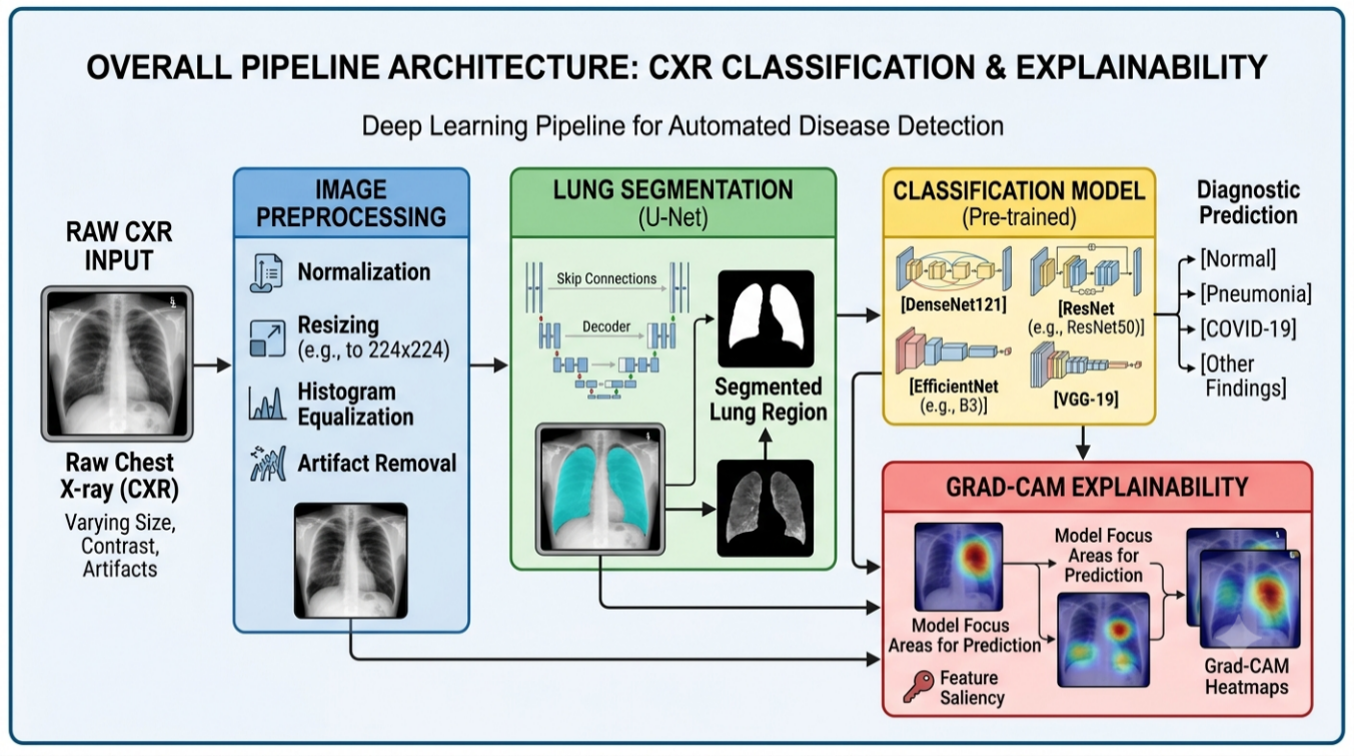
\includegraphics[width=\linewidth]{assets/chest1.png}
	\caption{Overall architecture of the proposed chest disease multi-class classification system, illustrating the sequential pipeline from raw CXR acquisition through preprocessing, lung segmentation, deep classification, and visual explainability.}
	\label{fig:chest_pipeline}
\end{figure}

\subsection{Dataset Description}
The classification system is trained, validated, and evaluated on a carefully curated composite dataset totaling \textbf{\num{17637} chest X-ray images} spanning four distinct diagnostic classes. This dataset is assembled from two complementary publicly available sources, described in detail below. A second, separate dataset is employed exclusively for training the lung segmentation model.

\subsubsection{Dataset 1: COVID-19 Radiography Database}
The \textbf{COVID-19 Radiography Database} is a landmark open-access collection assembled through a collaborative effort between researchers at Qatar University, the University of Dhaka, and partners in Pakistan and Malaysia, in cooperation with medical physicians. It was released on the Kaggle platform and has since become one of the most widely adopted benchmarks for COVID-19 CXR classification research.

The database contains chest radiographs in Portable Network Graphics (PNG) format at a resolution of 299×299 pixels, though images are resampled to 224×224 pixels during preprocessing. Each image is accompanied by a corresponding lung opacity mask, though these masks are not directly used in the classification training pipeline beyond informing the lung segmentation stage.

The COVID-19 subset of this database was compiled from multiple certified hospital sources and was expanded iteratively as more confirmed COVID-19 cases became publicly available. The radiographs represent a heterogeneous spectrum of COVID-19 severity, ranging from mild bilateral ground-glass opacities in early infection to extensive bilateral consolidation in severe and critical cases. Key radiological features visible in this subset include:

\begin{itemize}
	\item Bilateral, predominantly peripheral ground-glass opacities (GGO), often with a lower-zone preponderance.
	\item Multifocal consolidations with ill-defined margins.
	\item Peripheral airspace opacification with a characteristic "white lung" appearance in severe cases.
	\item Relative sparing of the central lung zones in early-stage disease.
	\item Absence of pleural effusion in most cases, which distinguishes COVID-19 from many bacterial pneumonias.
\end{itemize}

The Normal class images within this database originate from patients who presented with non-pulmonary complaints and underwent CXR as part of routine workup, with no reported pulmonary pathology on radiological review. This subset contributes the largest class to the combined dataset, providing a robust representation of normal pulmonary anatomy across diverse patient demographics.

\subsubsection{Dataset 2: Chest X-Ray Multiclass Dataset with Non-X-Ray Anomalies}
The second source is a composite multi-institutional dataset curated specifically to facilitate the training of models for real-world, open-set clinical deployment. A distinguishing and clinically important property of this dataset is the deliberate inclusion of non-X-ray images --- photographs of everyday objects such as animals and bicycles --- alongside genuine chest radiographs. This design enables the training of models with robustness to out-of-distribution inputs and supports open-set recognition, whereby the model can identify inputs that do not belong to any known radiographic class. \textbf{Importantly, the non-X-ray class was excluded from our training pipeline}, as our system targets only genuine CXR inputs.

The dataset integrates chest radiographs from globally recognized institutional sources, as illustrated in Table~\ref{tab:chest_datasets}

\begin{table}[htbp]
	\centering
	\caption{Datasets Used for Chest Disease Detection}
	\label{tab:chest_datasets}
	\small
	\renewcommand{\arraystretch}{1.2}
	
	\begin{tabularx}{\textwidth}{|
			>{\raggedright\arraybackslash}X|
			>{\raggedright\arraybackslash}X|
			>{\raggedright\arraybackslash}X|
			>{\raggedright\arraybackslash}X|}
		\hline
		\textbf{Source} & \textbf{Class(es)} & \textbf{Volume} & \textbf{Notes} \\
		\hline
		
		OCT Dataset (Kermany et al.) &
		Pneumonia, Normal &
		4,273 Pneumonia + 1,583 Normal &
		Pediatric and adult CXRs \\
		\hline
		
		RSNA CXR Dataset &
		Tuberculosis &
		1,750 TB-positive + 4,560 Normal &
		Radiological Society of North America \\
		\hline
		
		NIAID TB Dataset &
		Tuberculosis &
		1,300 TB-positive &
		Seven-country cohort \\
		\hline
		
		NLM Montgomery Dataset &
		TB, Normal &
		57 TB + 80 Normal (137 total) &
		Montgomery County, USA \\
		\hline
		
		NLM Shenzhen Dataset &
		TB, Normal &
		336 TB + 326 Normal (662 total) &
		Shenzhen No.3 Hospital, China \\
		\hline
		
		Belarus Dataset &
		Tuberculosis &
		304 TB-positive &
		512 $\times$ 512 px resolution \\
		\hline
		
		Non-X-ray Dataset (Sanagapati) &
		Non-X-ray (excluded) &
		1,357 object images &
		Not used in training \\
		\hline
		
	\end{tabularx}
\end{table}

This dataset is particularly valuable for the Tuberculosis and Pneumonia classes, which are otherwise under-represented in many COVID-19-centric benchmarks. The multi-national origin of the TB images ensures broad geographic and demographic coverage, lending the trained model greater generalizability across different patient populations and X-ray acquisition protocols.

\subsubsection{Combined Dataset and Class Distribution}
After merging both source datasets, applying quality filtering, and removing non-X-ray images, the final combined dataset comprises \textbf{\num{17637} images} distributed across four diagnostic classes. The dataset is partitioned into mutually exclusive training, validation, and test splits following standard machine learning practice.

The training set, used for gradient-based parameter optimization, contains \textbf{\num{15229} images} distributed across the four classes as shown in Table~\ref{tab:class_distribution}.

\begin{table}[htbp]
	\centering
	\caption{Class Distribution in the Training Dataset}
	\label{tab:class_distribution}
	\renewcommand{\arraystretch}{1.2}
	\begin{tabular}{|l|c|c|}
		\hline
		\textbf{Class} & \textbf{Number of Images} & \textbf{Proportion (\%)} \\
		\hline
		Normal & 4,870 & 31.98 \\
		\hline
		Pneumonia & 4,221 & 27.72 \\
		\hline
		COVID-19 & 3,192 & 20.96 \\
		\hline
		Tuberculosis & 2,946 & 19.34 \\
		\hline
		\textbf{Total (Training)} & \textbf{15,229} & \textbf{100.00} \\
		\hline
	\end{tabular}
\end{table}

The remaining approximately \textbf{\num{2408} images} are equally divided between the validation set (used for hyperparameter tuning and early stopping) and the held-out test set (used solely for final performance evaluation). This ensures that the reported test metrics reflect true generalization performance on unseen data.

Figure~\ref{fig:chest_images} presents representative sample radiographs from each of the four diagnostic classes, illustrating the distinctive visual characteristics and the degree of inter-class similarity that the classification model must learn to resolve.

\begin{figure}[htbp]
	\centering
	
	% First row
	\begin{subfigure}[b]{0.45\textwidth}
		\centering
		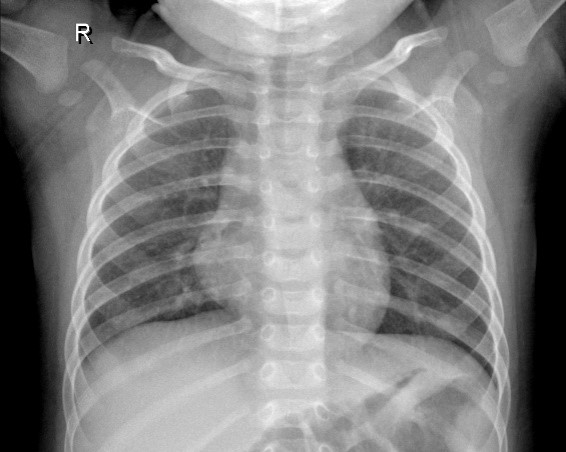
\includegraphics[width=\textwidth]{assets/chest2.jpg}
		\caption{Normal Chest X-ray}
		\label{fig:normal}
	\end{subfigure}
	\hfill
	\begin{subfigure}[b]{0.45\textwidth}
		\centering
		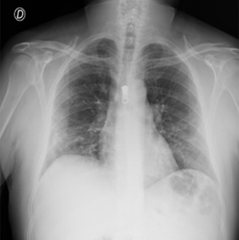
\includegraphics[width=\textwidth]{assets/chest4.png}
		\caption{COVID-19}
		\label{fig:covid19}
	\end{subfigure}
	
	\vspace{0.5cm}
	
	% Second row
	\begin{subfigure}[b]{0.45\textwidth}
		\centering
		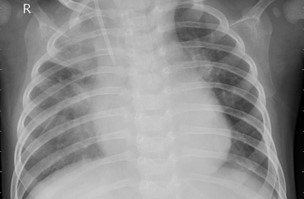
\includegraphics[width=\textwidth]{assets/chest3.jpg}
		\caption{Pneumonia}
		\label{fig:pneumonia}
	\end{subfigure}
	\hfill
	\begin{subfigure}[b]{0.45\textwidth}
		\centering
		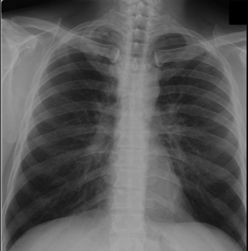
\includegraphics[width=\textwidth]{assets/chest5.png}
		\caption{Tuberculosis}
		\label{fig:tuberculosis}
	\end{subfigure}
	
	\caption{Representative chest radiograph samples from each of the four target diagnostic classes. The subtle visual differences between COVID-19 and Pneumonia are clear, underscoring the difficulty of the classification task.}
	\label{fig:chest_images}
\end{figure}

\subsubsection{Image Preprocessing Pipeline}
\label{sec:chest_preprocess}

Raw chest radiographs exhibit considerable variability in acquisition parameters, scanner characteristics, patient positioning, and image quality. To mitigate these sources of variability and produce a consistent, standardized input representation, all images undergo a three-stage preprocessing pipeline prior to training and inference. The preprocessing function is implemented in Python using the OpenCV library and is applied uniformly to all training, validation, and test images.

\paragraph{Step 1: Greyscale Loading}
All images are loaded in grayscale mode, discarding any color channels that may be present in saved PNG or JPEG files. Chest radiographs are inherently grayscale imaging modalities; the single luminance channel contains all diagnostically relevant information.

\paragraph{Step 2: Contrast Limited Adaptive Histogram Equalization (CLAHE)}
Standard global histogram equalization can over-amplify noise in homogeneous regions and create unnatural-looking artefacts. CLAHE addresses this by dividing the image into a grid of small, non-overlapping tiles (tile grid size of $8 \times 8$ pixels in this implementation) and applying histogram equalisation independently within each tile. A clip limit of $2.0$ is applied to prevent excessive contrast amplification. The CLAHE-enhanced image $\hat{I}$ is computed as:

\begin{equation}
	\hat{I}(x,y) =
	\mathrm{CLAHE}
	\left(
	I(x,y);
	\text{clipLimit}=2.0,\,
	\text{tileGrid}=8 \times 8
	\right)
	\label{eq:clahe}
\end{equation}

CLAHE is particularly effective at enhancing subtle infiltrates and opacities in lung tissue without washing out the finer structural details such as bronchial markings and vascular shadows, both of which carry diagnostic significance for tuberculosis and pneumonia detection.

\paragraph{Step 3: Gaussian Smoothing}
A Gaussian blur with a $5 \times 5$ kernel and automatically determined standard deviation ($\sigma = 0$, which causes OpenCV to compute $\sigma$ from the kernel size) is applied to suppress high-frequency noise introduced or amplified by the CLAHE step. The smoothed image is given by:

\begin{equation}
	I_{\mathrm{smooth}}(x,y)
	=
	I_{\mathrm{CLAHE}}(x,y) * G(x,y;\sigma)
	\label{eq:gaussian_blur}
\end{equation}

where

\begin{equation}
	G(x,y;\sigma)
	=
	\frac{1}{2\pi\sigma^{2}}
	\exp\left(
	-\frac{x^{2}+y^{2}}{2\sigma^{2}}
	\right)
	\label{eq:gaussian_kernel}
\end{equation}

denotes the two-dimensional Gaussian kernel, and $*$ denotes the convolution operation.

\paragraph{Step 4: Min-Max Normalization}
The smoothed image is normalized to the continuous floating-point range $[0,1]$:

\begin{equation}
	I_{\mathrm{norm}}(x,y)
	=
	\frac{I_{\mathrm{smooth}}(x,y)-I_{\min}}
	{I_{\max}-I_{\min}}
	\label{eq:normalization}
\end{equation}

This step ensures that all input pixel values lie within a consistent numerical range, which is a prerequisite for stable gradient-based optimization and consistent behavior across heterogeneous source datasets.

\paragraph{Greyscale to RGB Conversion}
The normalized single-channel image is converted to a three-channel RGB image by replicating the luminance channel across all three color channels. This step is necessary because the pre-trained backbone architectures (e.g., DenseNet121, ResNet50, and related models) are trained on the ImageNet dataset and therefore expect three-channel RGB inputs of size $224 \times 224 \times 3$.

The preprocessed images are saved as 8-bit unsigned integers, with pixel values scaled back to the range $[0,255]$ prior to storage, in the corresponding output directory. The original filename and directory structure are preserved to maintain dataset traceability and compatibility with subsequent processing stages.

Figures~\ref{fig:pneumonia_preprocessing} and~\ref{fig:tb_preprocessing} illustrate the effect of the preprocessing pipeline on representative Pneumonia and Tuberculosis radiographs, respectively.

\begin{figure}[htbp]
	\centering
	% First row
	\begin{subfigure}[b]{0.45\textwidth}
		\centering
		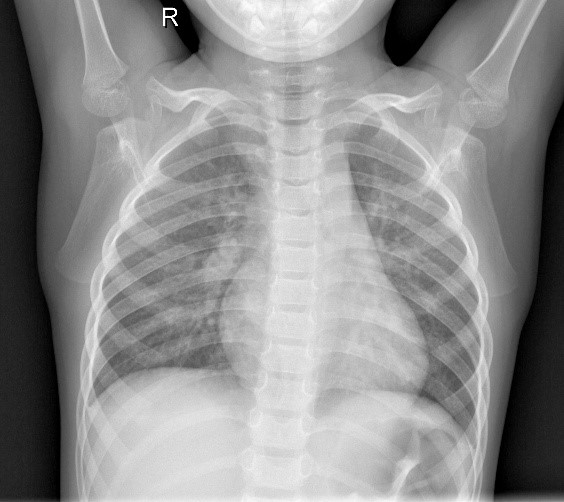
\includegraphics[width=\textwidth]{assets/chest6.jpg}
	\end{subfigure}
	\hfill
	\begin{subfigure}[b]{0.45\textwidth}
		\centering
		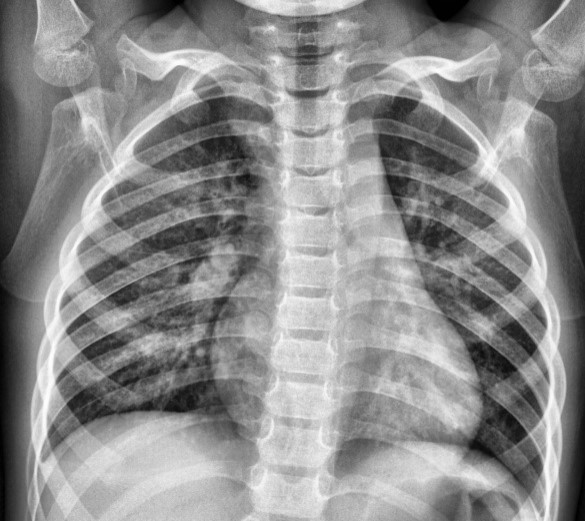
\includegraphics[width=\textwidth]{assets/chest7.jpg}
	\end{subfigure}
	\caption{Comparison of a Pneumonia chest radiograph before (left) and after (right).}
	\label{fig:pneumonia_preprocessing}
\end{figure}

\begin{figure}[htbp]
	\centering
	% First row
	\begin{subfigure}[b]{0.45\textwidth}
		\centering
		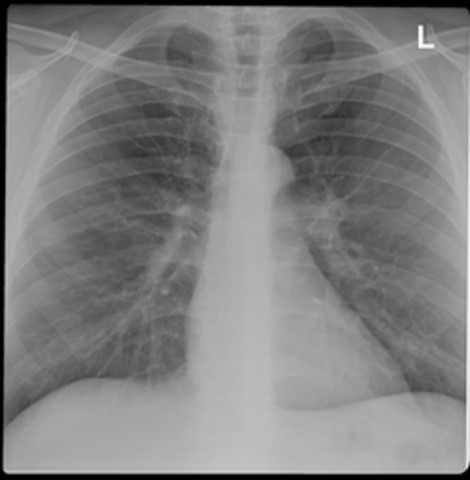
\includegraphics[width=\textwidth]{assets/chest8.jpg}
	\end{subfigure}
	\hfill
	\begin{subfigure}[b]{0.45\textwidth}
		\centering
		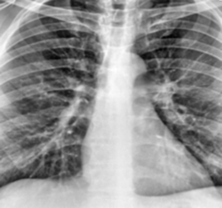
\includegraphics[width=\textwidth]{assets/chest9.png}
	\end{subfigure}
	\caption{Comparison of a Tuberculosis chest radiograph before (left) and after (right) the preprocessing pipeline.}
	\label{fig:tb_preprocessing}
\end{figure}

\subsubsection{Lung Segmentation Dataset}
A separate dataset is employed exclusively for training the U-Net lung segmentation model. This dataset is a curated combination of three well-established lung segmentation benchmarks: the \textbf{Darwin, Montgomery, and Shenzhen} datasets, with a combined total of \num{6810} image–mask pairs. Only the \textbf{Darwin subset (\num{6106} images and corresponding binary masks)} is used in the final segmentation training pipeline, as it provides the largest and most diverse collection.

Key characteristics of the Darwin dataset are:
\begin{itemize}
	\item Images include most of the cardiac shadow, exposing lung opacities that may be concealed behind the heart — a property of relevance for assessing viral pneumonia severity.
	\item Image resolutions, sources, and orientations vary significantly, ranging from $156 \times 156$ to $5600 \times 4700$ pixels, providing excellent scale invariance for training the segmentation model.
	\item Portable (bedside) X-ray images of significantly lower technical quality are included, enhancing the model's robustness to real-world image quality variability.
	\item Lung boundary annotations were generated using Darwin's Auto-Annotate AI tool and subsequently reviewed and corrected by expert radiologists, ensuring high annotation quality.
	\item The dataset does not contain lateral projection images; only PA/AP views are included.
\end{itemize}

Figure~\ref{fig:segmenation} presents an example image–mask pair from the Darwin segmentation dataset. The binary mask precisely delineates the left and right lung fields, including the lower-most visible portion defined by the diaphragmatic contour.

\begin{figure}[htbp]
	\centering
	% First row
	\begin{subfigure}[b]{0.45\textwidth}
		\centering
		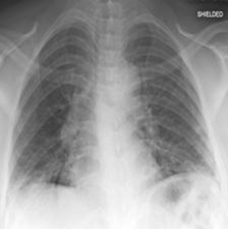
\includegraphics[width=\textwidth]{assets/chest10.png}
	\end{subfigure}
	\hfill
	\begin{subfigure}[b]{0.45\textwidth}
		\centering
		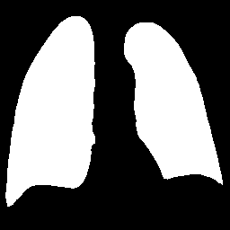
\includegraphics[width=\textwidth]{assets/chest11.png}
	\end{subfigure}
	\caption{Representative image–mask pair from the Darwin lung segmentation dataset. The mask precisely delineates both lung fields including regions behind the cardiac shadow.}
	\label{fig:segmenation}
\end{figure}

\subsection{Segmentation Model Details}
\label{sec:segmentation}
\subsubsection{Rationale for Lung Segmentation}
The inclusion of a dedicated lung segmentation preprocessing stage is a deliberate architectural decision grounded in both technical and clinical considerations. In a raw chest radiograph, the pulmonary fields of interest are surrounded by a rich context of non-pulmonary structures — the rib cage, thoracic spine, clavicles, cardiac silhouette, subdiaphragmatic organs, and soft tissues of the chest wall. From a pattern-recognition perspective, these structures can act as confounding variables: a CNN attempting to classify a COVID-19 image might inadvertently learn to exploit spurious correlations between disease prevalence and, for example, the projection angle or patient body habitus as reflected in bony structures, rather than developing genuine pathology-discriminative features.

By applying the segmentation mask prior to classification, the input to the classifier is restricted to the lung parenchyma, compelling the network to focus exclusively on pulmonary features. This masking strategy has been shown in the literature to improve classification specificity and reduce the likelihood of shortcut learning, particularly for conditions with subtle or distributed radiological findings such as COVID-19 and miliary TB.

\subsubsection{U-Net Architecture}
The lung segmentation model is built upon the \textbf{U-Net} architecture, originally proposed by Ronneberger, Fischer, and Brox (2015) for biomedical image segmentation tasks. U-Net is characterized by its distinctive encoder–decoder structure with lateral skip connections, which enables it to simultaneously capture high-level semantic context (through \textbf{the encoder's down sampling path}) and recover precise spatial localization detail (through the \textbf{decoder's up sampling path} and \textbf{skip connections}).

The implemented U-Net is designed to operate on grayscale images of size $224 \times 224 \times 1$ and produce a binary segmentation mask of identical spatial dimensions. The architecture is deliberately kept lightweight, with the encoder beginning at 32 filters to maintain computational efficiency while preserving sufficient representational capacity for the lung segmentation task. The complete architecture is described below.

\paragraph{Convolutional Block}
The fundamental building block of both the encoder and decoder paths is the convolutional block, which applies two successive $3 \times 3$ convolutions, each followed by Batch Normalization and ReLU activation:

\begin{equation}
	\mathrm{conv\_block}(x, F)
	=
	\mathrm{ReLU}\Big(
	\mathrm{BN}\big(
	\mathrm{Conv}_{3 \times 3}(
	\mathrm{ReLU}(
	\mathrm{BN}(\mathrm{Conv}_{3 \times 3}(x, F))
	)
	)\big), F
	\Big)
	\label{eq:conv_block}
\end{equation}

where $F$ denotes the number of output feature maps and $\mathrm{BN}$ denotes the Batch Normalization operation. The use of Batch Normalisation accelerates training convergence and acts as a regularizer, reducing dependence on precise weight initialization.

\paragraph{Encoder (Contracting Path)}
The encoder consists of four sequential encoder blocks, each comprising a convolutional block followed by a $2 \times 2$ max pooling operation with stride 2. Each encoder block produces two outputs: the feature map $s_i$ (skip connection) and the downsampled map $p_i$ (passed to the next encoder block):

\begin{equation}
	s_i = \mathrm{conv\_block}(p_{i-1}, F_i), \quad
	p_i = \mathrm{MaxPool}_{2 \times 2}(s_i)
	\label{eq:encoder_block}
\end{equation}

The filter counts at successive encoder levels are $F_1 = 32$, $F_2 = 64$, $F_3 = 128$, and $F_4 = 256$. After four pooling operations, the spatial resolution is reduced from $224 \times 224$ to $14 \times 14$.

\paragraph{Bridge (Bottleneck)}
The bridge layer connects the encoder and decoder without any pooling, applying a convolutional block with $F_5 = 512$ filters to the output of the deepest encoder level:

\begin{equation}
	b = \mathrm{conv\_block}(p_4, 512)
	\label{eq:bridge_layer}
\end{equation}

\paragraph{Decoder (Expansive Path)}
The decoder comprises four decoder blocks, each of which performs bilinear $2 \times 2$ upsampling, concatenates the upsampled feature map with the corresponding skip connection from the encoder, and applies a convolutional block:

\begin{equation}
	d_i =
	\mathrm{conv\_block}\Big(
	\mathrm{Concat}\big[
	\mathrm{UpSample}_{2 \times 2}(d_{i-1}),\, s_{5-i}
	\big],\, F_{5-i}
	\Big)
	\label{eq:decoder_block}
\end{equation}

The skip connections serve the critical function of restoring fine spatial detail that is inevitably lost during the max-pooling operations of the encoder. Without skip connections, the decoder would be forced to hallucinate precise boundary locations from the low-resolution bottleneck representation alone.

\paragraph{Output}
The final layer is a $1 \times 1$ convolutional layer with a single output channel and sigmoid activation, which maps the decoder's feature maps to a probability mask $\hat{M} \in [0,1]^{224 \times 224}$, where each value represents the probability of the corresponding pixel belonging to the lung region:

\begin{equation}
	\hat{M}(x,y)
	=
	\sigma\big(\mathrm{Conv}_{1 \times 1}(d_4)\big)
	=
	\frac{1}{1 + e^{-\mathrm{Conv}_{1 \times 1}(d_4)(x,y)}}
	\label{eq:final_output}
\end{equation}

The full encoder–decoder filter progression is summarized in Table~\ref{tab:unet_arch} and the complete U-Net architecture with tensor dimensions at each level is illustrated in Figure~\ref{fig:unet_arch}.

\begin{table}[htbp]
	\centering
	\caption{U-Net encoder–decoder filter progression and spatial resolutions (input: $224 \times 224 \times 1$).}
	\label{tab:unet_arch}
	\renewcommand{\arraystretch}{1.2}
	\begin{tabular}{|l|l|c|c|}
		\hline
		\textbf{Level} & \textbf{Block Type} & \textbf{Filters} & \textbf{Output Spatial Size} \\
		\hline
		Encoder 1 & conv\_block + MaxPool & 32  & $224 \times 224 \rightarrow 112 \times 112$ \\
		\hline
		Encoder 2 & conv\_block + MaxPool & 64  & $112 \times 112 \rightarrow 56 \times 56$ \\
		\hline
		Encoder 3 & conv\_block + MaxPool & 128 & $56 \times 56 \rightarrow 28 \times 28$ \\
		\hline
		Encoder 4 & conv\_block + MaxPool & 256 & $28 \times 28 \rightarrow 14 \times 14$ \\
		\hline
		Bridge & conv\_block & 512 & $14 \times 14$ \\
		\hline
		Decoder 1 & UpSample + Concat + conv\_block & 256 & $28 \times 28$ \\
		\hline
		Decoder 2 & UpSample + Concat + conv\_block & 128 & $56 \times 56$ \\
		\hline
		Decoder 3 & UpSample + Concat + conv\_block & 64  & $112 \times 112$ \\
		\hline
		Decoder 4 & UpSample + Concat + conv\_block & 32  & $224 \times 224$ \\
		\hline
		Output & Conv $1 \times 1$ + Sigmoid & 1 & $224 \times 224$ \\
		\hline
	\end{tabular}
\end{table}

\begin{figure}[htbp]
	\centering
	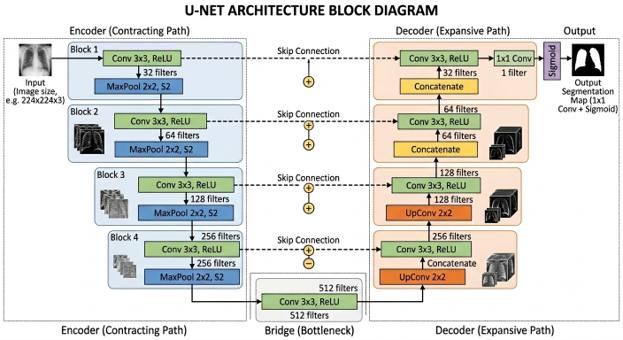
\includegraphics[width=\linewidth]{assets/chest12.png}
	\caption{U-Net architecture implemented for lung segmentation. The contracting path (left) captures contextual information through successive down sampling, while the expansive path (right) enables precise localization via skip connections. Tensor shapes are annotated at each level.}
	\label{fig:unet_arch}
\end{figure}
\FloatBarrier
\subsubsection{Loss Functions}
A compound loss function is employed for training the segmentation model, combining Binary Cross-Entropy (BCE) loss and Dice loss. This compound formulation simultaneously optimizes pixel-level probability calibration (via BCE) and the overlap between predicted and ground-truth masks (via Dice), yielding more stable training behavior and improved performance on the class-imbalanced segmentation task, where background pixels vastly outnumber lung pixels.

\textbf{Dice Coefficient:} The Dice Similarity Coefficient (DSC) measures the degree of overlap between the predicted mask $\hat{M}$ and the ground-truth mask $M$:

\begin{equation}
	\mathrm{DSC}(M,\hat{M}) =
	\frac{2 \sum_{i,j} M_{ij}\hat{M}_{ij} + \varepsilon}
	{\sum_{i,j} M_{ij} + \sum_{i,j} \hat{M}_{ij} + \varepsilon}
	\label{eq:dice_coefficient}
\end{equation}

where $\varepsilon = 1$ is a smoothing constant that prevents division by zero and improves gradient stability in early training epochs. The Dice coefficient ranges from 0 (no overlap) to 1 (perfect overlap).

\textbf{Dice Loss:}

\begin{equation}
	\mathcal{L}_{\mathrm{Dice}} = 1 - \mathrm{DSC}(M,\hat{M})
	\label{eq:dice_loss}
\end{equation}

\textbf{Binary Cross-Entropy Loss:} Applied pixel-wise across the entire image:

\begin{equation}
	\mathcal{L}_{\mathrm{BCE}} =
	-\frac{1}{N} \sum_{i,j}
	\Big[
	M_{ij} \log(\hat{M}_{ij}) +
	(1 - M_{ij}) \log(1 - \hat{M}_{ij})
	\Big]
	\label{eq:bce_loss}
\end{equation}

where $N$ is the total number of pixels per image.

\textbf{Combined Loss:}

\begin{equation}
	\mathcal{L}_{\mathrm{total}} =
	\mathcal{L}_{\mathrm{BCE}} + \mathcal{L}_{\mathrm{Dice}}
	\label{eq:total_loss}
\end{equation}

\subsubsection{Training Configurations}
The U-Net segmentation model is trained with the configuration shown in Table~\ref{tab:unet_training_config}extracted directly from the implementation.

\begin{table}[H]
	\centering
	\caption{U-Net segmentation model training configuration.}
	\label{tab:unet_training_config}
	\small
	\renewcommand{\arraystretch}{1.2}
	
	\begin{tabularx}{\textwidth}{|
			>{\raggedright\arraybackslash}p{0.35\textwidth}|
			>{\raggedright\arraybackslash}X|}
		\hline
		\textbf{Hyperparameter} & \textbf{Value} \\
		\hline
		
		Input shape & $224 \times 224 \times 1$ (grayscale) \\
		\hline
		
		Batch size & 8 \\
		\hline
		
		Initial epochs (Phase 1) & 10 \\
		\hline
		
		Fine-tuning epochs (Phase 2) & 4 \\
		\hline
		
		Optimizer & Adam \\
		\hline
		
		Learning rate & $1 \times 10^{-4}$ \\
		\hline
		
		Loss function & BCE + Dice (combined) \\
		\hline
		
		Evaluation metric & Dice Coefficient, Accuracy \\
		\hline
		
		Early stopping monitor &
		\texttt{val\_dice\_coef} (patience = 5, mode = max) \\
		\hline
		
		LR reduction &
		ReduceLROnPlateau (factor = 0.1, patience = 5, min LR = $1 \times 10^{-7}$) \\
		\hline
		
		Precision policy &
		Mixed float16 (TensorFlow AMP) \\
		\hline
		
		Training / validation split &
		85\% / 15\% (6,106 Darwin images) \\
		\hline
		
		Best model checkpoint &
		\texttt{lung\_segmentation\_darwin\_montgomery\_shenzhen.h5} \\
		\hline
		
	\end{tabularx}
\end{table}

The dataset is shuffled with a fixed seed of 42 before splitting to ensure reproducibility. The training loop uses data pipelines with prefetching to maximize GPU utilization. Mixed float16 precision is enabled via TensorFlow's Automatic Mixed Precision (AMP) to accelerate training on modern NVIDIA GPU architectures with Tensor Core support.

A two-phase training strategy is adopted: in Phase 1, the model is trained from a random initialization for 10 epochs to establish stable feature representations. In Phase 2, the best Phase 1 checkpoint (\texttt{lung\_segmentation\_final\_v2.h5}) is reloaded and fine-tuned for a further 4 epochs at the same learning rate, allowing the model to refine its lung boundary delineation capability. The best overall weights --- measured by \texttt{val\_dice\_coef} ---are saved as the final segmentation model.

\begin{figure}[htbp]
	\centering
	
	% First row
	\begin{subfigure}[b]{0.45\textwidth}
		\centering
		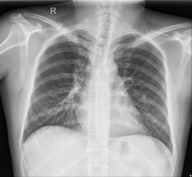
\includegraphics[width=\textwidth]{assets/chest13.png}
		\caption{Original}
	\end{subfigure}
	\hfill
	\begin{subfigure}[b]{0.45\textwidth}
		\centering
		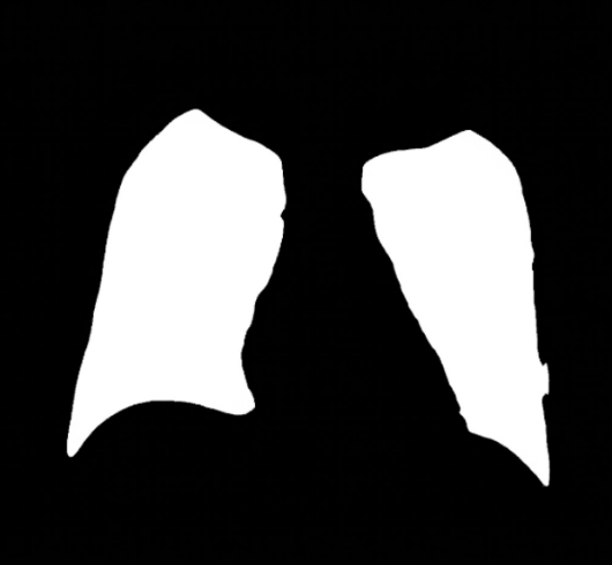
\includegraphics[width=\textwidth]{assets/chest14.png}
		\caption{Binary Mask}
	\end{subfigure}
	
	\vspace{0.5cm}
	
	% Second row
	\begin{subfigure}[b]{0.45\textwidth}
		\centering
		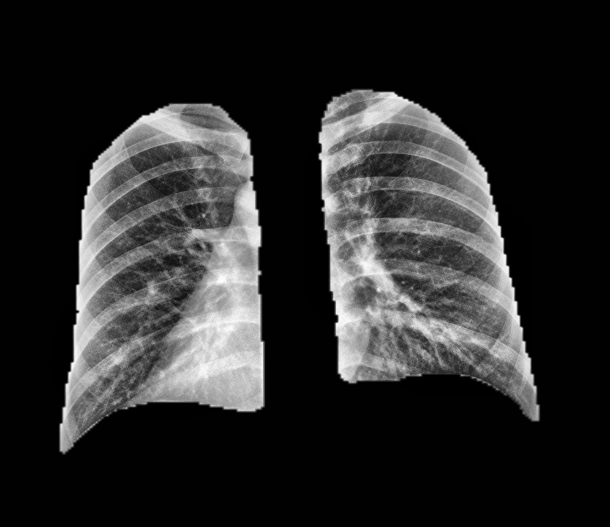
\includegraphics[width=\textwidth]{assets/chest15.png}
		\caption{Segmented Image}
	\end{subfigure}
	
	\caption{U-Net segmentation results. From left to right: the preprocessed input radiograph, the predicted binary lung mask, and the masked output image passed to the classification stage.}
	\label{fig:segmentation_example}
\end{figure}

\subsubsection{Classification Model: DenseNet121 with One-vs-Rest (OVR)}
The primary classification backbone is DenseNet121 (Densely Connected Convolutional Networks, Huang et al., 2017), a 121-layer deep CNN pre-trained on the ImageNet dataset. DenseNet121 is particularly well-suited for medical image classification for several reasons:

\begin{itemize}
	\item \textbf{Dense connectivity:} Each layer receives feature maps from all preceding layers, enabling maximum feature reuse and gradient flow. This alleviates the vanishing gradient problem and allows effective training even with relatively limited medical imaging datasets.
	
	\item \textbf{Parameter efficiency:} Dense connectivity reduces the number of required parameters compared to conventional deep networks of comparable performance, reducing the risk of overfitting on limited data.
	
	\item \textbf{Multi-scale feature aggregation:} The dense connections allow the final layers to simultaneously access low-level texture features and high-level semantic representations, which is advantageous for the heterogeneous visual patterns of different chest pathologies.
\end{itemize}

The model follows a transfer learning approach with partial fine-tuning. The DenseNet121 feature extractor is initialized with ImageNet pre-trained weights, and the last 100 layers are made trainable while all earlier layers are frozen. This selective fine-tuning strategy preserves the low-level and mid-level representations learned from ImageNet (edges, textures, simple patterns) whilst allowing task-specific adaptation of higher-level representations through gradient updates.

A custom classification head is appended to the Global Average Pooling (GAP) output of the base model. The GAP operation reduces the spatial feature map to a 1024-dimensional feature vector, eliminating the need for large fully connected layers and thereby reducing parameters and overfitting risk. The head architecture is:

\begin{equation}
	z =
	\mathrm{Dropout}_{0.3}
	\Big(
	\mathrm{Dense}_{256}^{\mathrm{ReLU}}
	\big(
	\mathrm{Dropout}_{0.4}
	(\mathrm{Dense}_{512}^{\mathrm{ReLU}}(\mathrm{BN}(\mathrm{GAP}(F))))
	\big)
	\Big)
	\label{eq:classification_head}
\end{equation}

\begin{equation}
	\hat{y} = \sigma(W_{\mathrm{out}} z + b_{\mathrm{out}}),
	\quad
	\hat{y}_k = \frac{1}{1 + e^{-(W_k z + b_k)}}
	\label{eq:ovr_output}
\end{equation}

where $F$ denotes the final convolutional feature map of DenseNet121, $\mathrm{GAP}(\cdot)$ denotes Global Average Pooling, $\mathrm{BN}(\cdot)$ denotes Batch Normalization, and $\sigma(\cdot)$ denotes the sigmoid activation. Each of the $K = 4$ output neurons operates as an independent binary classifier, producing a probability score $\hat{y}_k \in [0,1]$ for each class $k$.

This One-vs-Rest (OVR) multi-label formulation with sigmoid output offers several advantages over a conventional SoftMax multi-class formulation. In the SoftMax approach, the probabilities of all classes are coupled (they must sum to one), which can suppress the activation of a class when multiple classes co-occur or when the model is uncertain. With sigmoid, each class is modeled independently, allowing the model to assign high confidence to multiple classes simultaneously when the image features are ambiguous or the pathology is mixed.

The model architecture is illustrated in Figure~\ref{fig:chest_model_arch1}.
\begin{figure}[H]
	\centering
	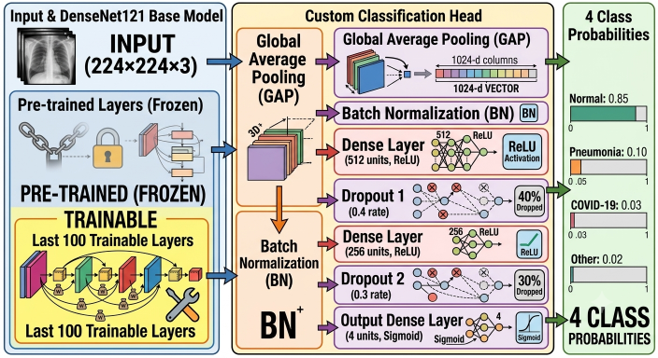
\includegraphics[width=\linewidth]{assets/chest16.png}
	\caption{Proposed DenseNet121 OVR classification model architecture. The base network produces a 1024-dimensional feature vector via Global Average Pooling, which is refined through the custom classification head before producing independent sigmoid probability scores for each diagnostic class.}
	\label{fig:chest_model_arch1}
\end{figure}

The training employs Binary Cross-Entropy (BCE) loss rather than categorical cross-entropy, consistent with the OVR formulation where each class is an independent binary classification target. The BCE loss for a batch of $N$ samples with $K = 4$ classes is:

\begin{equation}
	\mathcal{L}_{\mathrm{BCE\text{-}OVR}} =
	-\frac{1}{N \cdot K}
	\sum_{n=1}^{N}
	\sum_{k=1}^{K}
	\Big[
	y_{nk} \log(\hat{y}_{nk}) +
	(1 - y_{nk}) \log(1 - \hat{y}_{nk})
	\Big]
	\label{eq:bce_ovr}
\end{equation}

Class imbalance is addressed through inverse-frequency class weights, computed as:

\begin{equation}
	w_k =
	\frac{N_{\mathrm{total}}}{K \cdot N_k}
	\label{eq:class_weights}
\end{equation}

where $N_{\mathrm{total}}$ is the total number of training samples and $N_k$ is the number of samples in class $k$.
\newpage
\subsection{Grad-CAM Integration}
\label{sec:chest_xai}
\subsubsection{Rationale for Explainability}
The deployment of any AI-based diagnostic tool in a clinical environment is inseparable from the question of trust and accountability. A classification model, however accurate its aggregate performance metrics, remains clinically unacceptable if its decision-making process is opaque and cannot be scrutinized by the responsible physician. The recognition of this challenge has given rise to the field of Explainable Artificial Intelligence (XAI), which encompasses a broad family of techniques aimed at rendering the internal reasoning of machine learning models interpretable to human observers.

In the context of medical imaging, XAI serves multiple critical functions:

\begin{itemize}
	\item \textbf{Verification of clinical validity:} Confirming that the model attends to medically meaningful regions (e.g., lung infiltrates for COVID-19) rather than spurious correlations (e.g., imaging artifacts or patient positioning markers).
	
	\item \textbf{Detection of shortcut learning:} Identifying cases where the model has learned to exploit non-clinical features present in the training data due to dataset biases.
	
	\item \textbf{Clinical decision support:} Providing the reporting radiologist with a visual ``second opinion'' that highlights the most diagnostically salient regions for each prediction.
	
	\item \textbf{Regulatory compliance:} Meeting the increasingly stringent interpretability requirements of medical device regulations in various jurisdictions.
\end{itemize}

\subsubsection{Gradient-weighted Class Activation Mapping (Grad-CAM)}
The chosen XAI technique is Grad-CAM (Gradient-weighted Class Activation Mapping), introduced by Selvaraju et al. (2017). Grad-CAM is a gradient-based localization method that produces a coarse spatial importance map $\hat{L}^c \in \mathbb{R}^{u \times v}$ for a target class $c$, indicating which spatial regions of the input image were most influential in driving the model's prediction for that class.

The Grad-CAM computation proceeds as follows for a target class $c$ and a chosen convolutional layer $A$ with $K$ feature maps $A^k \in \mathbb{R}^{u \times v}$:

\paragraph{Step 1: Compute Class-Discriminative Gradient}
The gradient of the class score $\hat{y}^c$ (the logit for class $c$ before the final sigmoid) with respect to the $k$-th feature map $A^k$ is computed via backpropagation through the final convolutional layer:

\begin{equation}
	\frac{\partial \hat{y}^c}{\partial A^k}
	\label{eq:gradcam_gradient}
\end{equation}

\paragraph{Step 2: Global Average Pool the Gradients}
The importance weight $\alpha_k^c$ for feature map $k$ with respect to class $c$ is obtained by spatially average pooling the gradients:

\begin{equation}
	\alpha_k^c =
	\frac{1}{Z}
	\sum_i \sum_j
	\frac{\partial \hat{y}^c}{\partial A_{ij}^k}
	\label{eq:gradcam_alpha}
\end{equation}

where $Z = u \times v$ is the number of spatial locations. Intuitively, $\alpha_k^c$ measures how sensitive the class-$c$ score is to changes in feature map $k$.

\paragraph{Step 3: Compute Weighted Combination and Apply ReLU}
The Grad-CAM heatmap is the ReLU-activated weighted sum of the feature maps:

\begin{equation}
	\hat{L}^c = \mathrm{ReLU}\left(\sum_k \alpha_k^c A^k \right)
	\label{eq:gradcam_heatmap}
\end{equation}

The ReLU operation retains only the features that have a positive influence on the target class score, discarding negative activations that correspond to features of other classes.

\paragraph{Step 4: Resize and Normalize}
The heatmap $\hat{L}^c \in \mathbb{R}^{u \times v}$ (typically $7 \times 7$ for the last DenseNet convolutional layer) is bilinearly resized to match the input image dimensions ($224 \times 224$) and normalized to the range $[0,1]$:

\begin{equation}
	\tilde{L}^c =
	\frac{L_{\mathrm{resized}}^c - \min(L_{\mathrm{resized}}^c)}
	{\max(L_{\mathrm{resized}}^c) - \min(L_{\mathrm{resized}}^c)}
	\label{eq:gradcam_normalization}
\end{equation}

\paragraph{Step 5: Color Mapping and Overlay}
The normalized heatmap is converted to a pseudo-color image using the JET color map (blue = low importance, red = high importance) and blended with the original RGB image at a mixing ratio of 0.4:0.6 to produce the final Grad-CAM visualization:

\begin{equation}
	I_{\mathrm{Grad\text{-}CAM}} =
	\mathrm{JET}(\tilde{L}^c)\times 0.4 + I_{\mathrm{orig}} \times 0.6
	\label{eq:gradcam_final}
\end{equation}

Values are clipped to $[0,255]$ and cast to 8-bit unsigned integers before display.

\subsubsection{OVR Grad-CAM for Multi-Class Visualization}
In the OVR model, each output neuron is an independent binary classifier. The Grad-CAM implementation accordingly generates a separate heatmap for each class whose predicted probability exceeds the decision threshold $\tau = 0.5$. If no class reaches the threshold, the class with the highest sigmoid score is selected as the target. The final visualization presents the original image alongside one Grad-CAM overlay per active class, enabling simultaneous visualization of multiple class-discriminative regions when the model detects co-occurring pathologies or is uncertain between classes.

The target convolutional layer for Grad-CAM is the final dense block concatenation layer of DenseNet121, accessed via the Keras layer name \texttt{conv5\_block16\_concat}. This layer produces feature maps at a spatial resolution of $7 \times 7$ with 1024 channels, providing a rich and discriminative representation just before the global pooling operation.

Samples from the process and the output are shown for representative samples from the pneumonia and Tuberculosis scans in Figure~\ref{fig:grad_cam_vis_pneumonia}, and Figure~\ref{fig:grad_cam_vis_tb} respectively.

\begin{figure}[H]
	\centering
	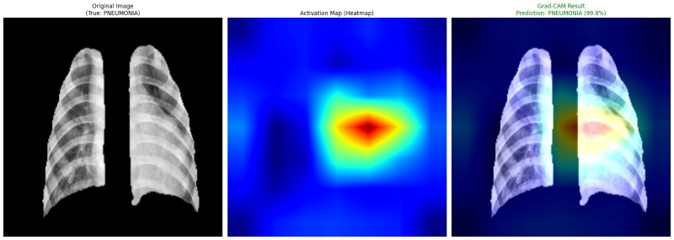
\includegraphics[width=\linewidth]{assets/chest17.jpg}
	\caption{Grad-CAM visualization results for Pneumonia representative case. The saliency maps confirm that the model attends to pathologically relevant lung regions.}
	\label{fig:grad_cam_vis_pneumonia}
\end{figure}

\begin{figure}[H]
	\centering
	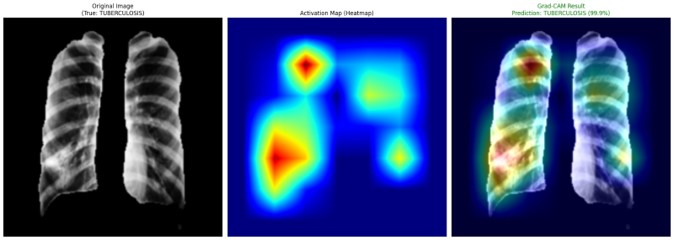
\includegraphics[width=\linewidth]{assets/chest18.jpg}
	\caption{Grad-CAM visualization results for Tuberculosis cases. The upper-lower lobe localization of saliency for TB cases confirms the model's ability to recognize TB-specific radiological patterns.}
	\label{fig:grad_cam_vis_tb}
\end{figure}

